\chapter{Methodology}
\label{chapter:methodology}

The methodology used for the study presented in this thesis consisted of five major steps. To gain a deeper understanding of the problem of information discovery and curation, (1) I conducted a systematic literature review. Based on the literature review, (2) I derived a preliminary set of information discovery and curation design factors and related them within a framework. (3) The framework was then applied for the evaluation of 20 different information discovery applications and iteratively refined after every evaluation. (4) The resulting framework was used to develop a novel place photo discovery application,revealing unforeseen gaps that were consequently addressed. Lastly, (5) the framework was applied to a reevaluation of some of the previously evaluated tools with the purpose of validating its effectiveness.  A summary of the methodology is presented in Figure~\ref{fig:methodology}.
\begin{figure}[ht!]
	\noindent
	\centering
    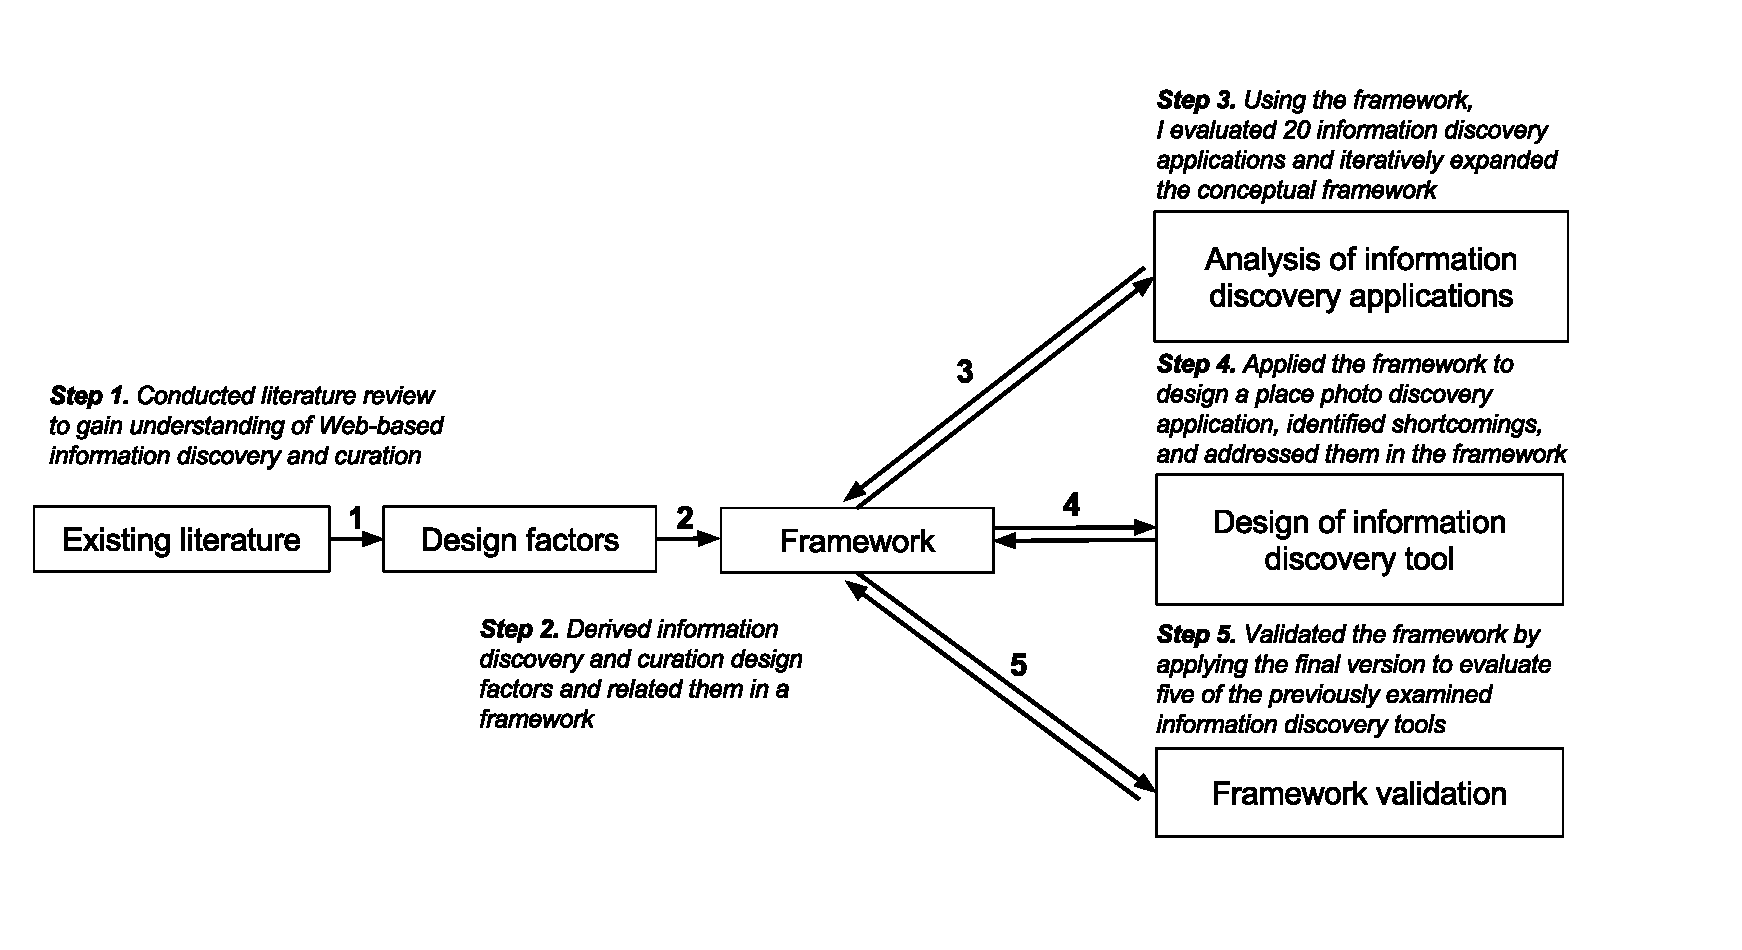
\includegraphics[width=\linewidth]{methodology.pdf}
	\caption{Methodology Overview}
	\label{fig:methodology} 
\end{figure}

{\section{Research Questions and Objective}
This study was designed to address the problem of designing Web applications for information discovery and was motivated by the following research questions:

\emph{RQ1:~How do existing Web applications support information discovery?}

\emph{RQ2:~How do existing information discovery applications support information curation?}

Using insights from RQ1 and RQ2 , my main research objective is the following:

\emph{RO:~To develop a framework for performing summative and formative evaluation of Web-based information discovery and curation tools.}


\pagebreak

To address RQ1 and RQ2, I conducted a systematic literature review (see Section~\ref{section:lit_review}) and a case study of 20 information discovery tools (see Section~\ref{section:building}). Using the insights that I learned from answering RQ1 and RQ2, I constructed a conceptual framework for information discovery and curation. (see Sections~\ref{section:building}, \ref{section:applying}, \ref{section:validating}). 
}% end section

{\section{Literature Review}
\label{section:lit_review}
The development of the framework began with an extensive literature review. A diverse set of topics contributed to forming an understanding of information discovery and curation, including information behaviour and information seeking models, high-level Web tasks and modes of Web use, exploration-based models of discovery, and methods of personal and social curation. From this review, the preliminary design factors for the framework were derived. Key findings in the current literature are presented in Chapter~\ref{chapter:chapter_related_work}.
}% end section

{\section{Building and Refining the Conceptual Framework}
\label{section:building}
Through a careful analysis of 20 information discovery applications (see Table~\ref{table:tools}), the framework was iteratively expanded by adding new concepts and establishing relations between those concepts.  The framework was refined as I explored the literature and available tools, and for presentation purposes in this thesis, I present only two versions of the framework. The preliminary framework was a result of this tool analysis and depicted in Chapter~\ref{chapter:old_framework}. The final version of the framework (see Chapter~\ref{chapter:framework}) was a result of developing an information discovery application based on the preliminary work.    

For my case study, I selected some of the most used information discovery applications today and considered the full range of features in those tools (both by referring to the literature and documentation on those tools, as well as exploring the features). The popularity of information discovery applications was determined using Website popularity ranks provided by Alexa\footnote[1]{Alexa is available at www.alexa.com}, a commercial Web traffic data provider. The focus was on applications that had strong information discovery components and lesser priority was given to applications whose purpose revolved only around curation.

I used Yin's strategies for designing a case study~\cite{yin2014case} for guidance. The motivation behind choosing a case study over other methods of qualitative research was based on my choice of research questions, the lack of control over existing applications and their development, and having to focus on contemporary use of real-life Web applications. According to Yin~\cite{yin2014case}, a case study would be an optimal research strategy given the above characteristics.

My study consisted of 20 cases, whereby each case is a Web application that focuses on the support of information discovery. I examined the overall purpose of each application, its description as defined within the application, as well as literature and documentation related to the application (if they were available) against the features that the application provided. For example, if an application provided bookmarking features, I checked if it was indeed intended to be used for information preservation. 

Consequently, the methodology was an iterative process of selecting cases, analyzing them, and determining whether they could be described and evaluated using the framework. If I found a key feature that could not be described, I adapted the framework according to the findings. I repeated the process of case selection and evaluation until the framework was usable for all cases. I then grouped the elements of the framework into categories, recording corresponding questions to ask in order to evaluate applications. 

A list of the tools that were used in this study are presented in Table~\ref{table:tools}. Summaries of their evaluations using the preliminary framework can be found in Appendix~\ref{chapter:appendix_tools}. Other tools were considered throughout the study, however, only the 20 applications presented underwent systematic examination. 

\begin{table*}[htbp]
\small
\label{table:tools}
\caption{Web-based Information Discovery and Curation Tools as of May 15, 2014}

\begin{tabular}{|p{0.20\linewidth}| p{0.30\linewidth}| p{0.45\linewidth}|}

\hline
\textbf{Application} & \textbf{Address} & \textbf{Description}
\\
\hline
Pinterest       & www.pinterest.com 	& Visual discovery tool \\
\hline
Delicious       & delicious.com 		& Social bookmarking service \\
\hline
Tumblr          & www.tumblr.com 		& Microblogging platform \\
\hline
StumbleUpon     & www.stumbleupon.com  	& Web page discovery tool \\
\hline
Wikipedia       & en.wikipedia.org   	& Free content Internet encyclopedia\\
\hline
Google Maps     & www.google.ca/maps  	& Web mapping service\\
\hline
Rotten Tomatoes & www.rottentomatoes.com & Movie and TV database\\
\hline
500px           & 500px.com            	& Photography site\\
\hline
BucketList      & bucketlist.org  		& Goal tracking and discovery service\\
\hline
We Heart It     & weheartit.com 		& Visual discovery tool \\
\hline
Scoop.it!       & www.scoop.it 			& Online publishing platform \\
\hline
Google Images   & images.google.com  	& Image discovery service \\
\hline
Vimeo           & vimeo.com  			& Video sharing Website\\
\hline
LifeHacker      & lifehacker.com        & Daily blog \\
\hline
YouTube         & www.youtube.com 		& Video hosting platform \\
\hline
Yelp            & www.yelp.ca  			& Business review site\\
\hline
IMDb            & www.imdb.com  		& Movie database \\
\hline
Trip Adviser    & www.tripadvisor.ca 	& Travel site \\
\hline
Urban Spoon     & www.urbanspoon.com    & Online bar and restaurant guide\\
\hline
Thesaurus       & thesaurus.com         & Online thesaurus \\
\hline
\end{tabular}
\end{table*}
} % end section
\pagebreak
{\section{Applying the Framework to the Design of an Information Discovery and Curation Application}
\label{section:applying}

In order to analyze the framework's capabilities when designing for information discovery and curation, I used the framework as a guide for developing a place photo discovery application. The motivation for choosing a place photo discovery application was based on the gaps that were exposed during analysis of some of the applications, such as Google Maps and Pinterest. Applying the framework to designing an application has triggered more changes within the framework, its further extension and refinement. The resulting application is discussed in Chapter~\ref{chapter:application}.
}% end section

{\section{Framework Validation}
\label{section:validating}
In order to further validate the framework, it was applied to the reevaluation of five of the previously examined tools (see Chapter~\ref{chapter:application}). For each tool, I identified gaps and proposed directions for future development. 
}% end section

{\section{Limitations}
The case study I conducted has a number of limitations. A lack of documentation, research literature, and formal descriptions of available features for some applications introduces a threat to the construct validity of the study. In addition, information discovery tools and features can be used in unintended or unforeseen ways by designers and developers. Therefore, the recorded use of some features within information discovery applications was recorded on my interpretations. To compensate for such limitations, I personally employed the tools over an extended period of time to gain a deeper understanding of their use. In addition, I considered some cases with similar functionality and design to be able to validate or clarify prior findings. 

Many Web applications evolve rapidly. Therefore, my tool analysis only applies to tools at the moment of the study.
\pagebreak

Only Web applications running in browsers on a desktop computer were considered in this study. The study can be extended with use of various devices, such as smartphones and tablets, as information discovery patterns and mechanisms may vary for different platforms. 

Another limitation was the lack of prior research on the subject matter. Some researchers have studied information seeking models and high-level Web tasks, but there is a lack of literature on how to enable and support different Web tasks. This opens up opportunities for future research to analyze methods of developing and building frameworks for facilitating and evaluating tools that support other Web tasks, such as communication, transactions, and goal realization.


} % end section

